
In EDGE, data is passed between blocks through reading and writing to general purpose registers.
To ensure that a younger block does not not execute a register read before an older block has executed a write to the same register, the register-file keeps track of registers which will be written to.
If the younger block attempts to execute the read, its request will be pushed back until the older block has executed its write.

\lstset{
	backgroundcolor=\color{lbcolor},
	tabsize=2,
	rulecolor=,
	language=matlab,
        basicstyle=\tiny,
        upquote=true,
        aboveskip={1\baselineskip},
        columns=fixed,
        showstringspaces=false,
        extendedchars=true,
        breaklines=true,
        prebreak = \raisebox{0ex}[0ex][0ex]{\ensuremath{\hookleftarrow}},
        frame=single,
        showtabs=false,
        showspaces=false,
        showstringspaces=false,
        identifierstyle=\ttfamily,
        keywordstyle=\color[rgb]{0,0,1},
        commentstyle=\color[rgb]{0.133,0.545,0.133},
        stringstyle=\color[rgb]{0.627,0.126,0.941},
		numbers=left,
}

\begin{figure}[t]
\lstset{language=C,numbersep=4pt}
\begin{center}
\begin{lstlisting}
for(int i = 0; i < 100000; i++)
         a[i]+= c[i] * b[i];
\end{lstlisting}
\end{center}
\vspace{-1em}
\captionof{lstlisting}{Very basic loop.}
\label{lst:chp3:small}
\vspace{1em}
\end{figure}

Whilst this ensures correct execution of speculative blocks, it effectively reduces the potential for instruction level parallelism (ILP).
This is further exacerbated when fusing cores, as this increases the amount of blocks that may potentially have to wait on register reads and writes.
For example, the loop iterator in Listing~\ref{lst:chp3:small} will be passed between iterations of the block through a register.
If multiple cores are composed, and all have an iteration of the loop, they may have to wait on previous writes to be able to execute their loads; serialising execution of the loop.

In situations where register dependencies are a bottleneck and cannot be optimised via a compiler, core composition cannot be considered an effective method of improving performance.
The problem of trying to reduce register and memory dependencies to improve instruction level parallelism is not new, and is an issue for more traditional superscalar processors.
In these cases value prediction can be used to attempt to ensure that these blocks can run in parallel even if there are dependencies.

\subsection{Implementation}

\subsubsection{Design features of a value predictor}

This section covers different features that must be considered when implementing a value predictor for the EDGE architecture.

\paragraph*{Prediction Latency} Before discussing the implemented value predictor in this chapter, it is important to explain why it was chosen.
In a traditional superscalar processor, one of the main challenges value predictors face is being able to sustain the potential number of prediction requests in a short time frame~\cite{peraisBeBop2015}.
As value predictors were designed to improve ILP performance of out-of-order (OoO) superscalars, it is important to be able to submit value predictions quickly.
If multiple prediction requests are made each cycle, this may require to add expensive hardware such as ***, which may dissuade designers from using value predictors.

To tackle the challenge of issuing predictions quickly, research has focussed on grouping instructions into prediction blocks~\cite{peraisBeBop2015}.
Instead of fetching a single prediction, the value predictor's tables are split into fixed groups of values.
In a traditional OoO processor, this method can be compared to fetching values for a basic block of instructions; it allows the predictor to issue multiple predictions at once.
However, in a traditional OoO this may be complicated by the fact that basic blocks have multiple entry points, and thus some extra hashing must be added to the predictor to ensure that the prediction blocks start at the correct instruction. % clarify
Finally, a block-based value predictor requires that the size of a block be determined at design time, which adds a new design task: choosing a small block size will increase the number of requests per cycle, whilst a large block size will decrease the number of entries and thus reduce overall accuracy. %clarify
Even so, as the EDGE ISA already organises instructions into blocks, a block-based value predictor is an attractive design.

\paragraph*{Prediction generation} Another important feature when selecting a value predictor is how it generates a predicted value.
As of the writing of this thesis, there exist two main methods: direct value prediction and stride-based value prediction.
The direct value predictor is the simpler design, as it only stores the last value for the specific register or memory address.
When a request is made, the direct value predictor will simply submit the last value.
Whilst this makes a value predictor small easy to design, such implementation is known to have poor accuracy when predicting values that are modified in quick succession.

On the other hand, stride-based value predictors use two components to make a prediction.
The first component is a Last-Value Table (LVT) which holds the last known value for a register or memory address.
The second component is a stride, which represents the difference between the last two values of the data.
Thus, when a prediction is made, the value predictor fetches the value from the LVT, and adds the stride to make a prediction.
Such a design may increase the memory footprint as it has to store both a value and a stride for each data point; however it improves the overall accuracy and usefulness of value predictors.

\subsection{Determining block size}

\begin{figure}[t]
    \centering
    \includegraphics[width=1\textwidth]{chapter3/graphics/averageRegRead.pdf}

    \caption{Average number of register reads and writes per EDGE block.}
    \label{fig:edge_reg_read}
	\vspace{1em}
\end{figure}

One of the defining factors of the block based D-VTAGE predictor is that a single prediction fetches a fix set of values rather than requiring one request per instruction.
Due to the fact that the block size is fixed, determining the correct size is important.
Having a large block size means that the D-VTAGE predictor can predict all values in a block, however this comes at the sacrifice of having less blocks in memory.
On the other hand, small block size allows to have multiple blocks stored at a time but may require values of an EDGE block to be found in multiple D-VTAGE blocks.
This would increase the number of requests to the value predictor, which may become a bottleneck.

In this chapter, the value predictor is focused on register reads rather than load-store operations.
This is due to the fact that, unless the load-store dependence predictor detects a data dependency between two blocks, memory operations operate in parallel.
Focussing only on register reads will reduce the the block size requirements as reads tend to be a minor component of an EDGE block.
To determine the block size, all the EDGE blocks of the SD-VBS benchmarks are anaylsed to find out the what the average register read and write count is per block.
The writes are also tracked as it provides information on the potential amount of register dependencies found in each of the applications.

Figure~\ref{fig:edge_reg_read} shows the average number of register read and writes for each of the benchmarks.
On average, there are 5 register reads and 3 register writes per block.
Whilst \bm{Disparity} \bm{Localization}, \bm{Texture\_Synthesis} and \bm{Tracking} have higher register read counts than the average, most of them only have 5 writes per block.
This potentially means that having a D-VTAGE block size of 5 would capture all dependencies.
However this would require some form of detecting which reg



\subsection{Perfect Value Predictor}

The perfect value predictor is implemented using traces of the application being executed.
When a new block is fetched, it querries the trace file and looks for the values of all the registers which will be read.
When the block can execute a read, the simulator then feeds the register directly into the instruction operands, instead of querying the register file.

The perfect value predictor has no hardware restriction as to fully capture the potential performance improvements.
Thus, all the registers in a block can be predicted.
More on how restricting the number of values which can be predicted per block is discussed in the analysis in Section~\ref{chp:chp3:sec:analysis}.

\begin{figure}[t]
    \centering
    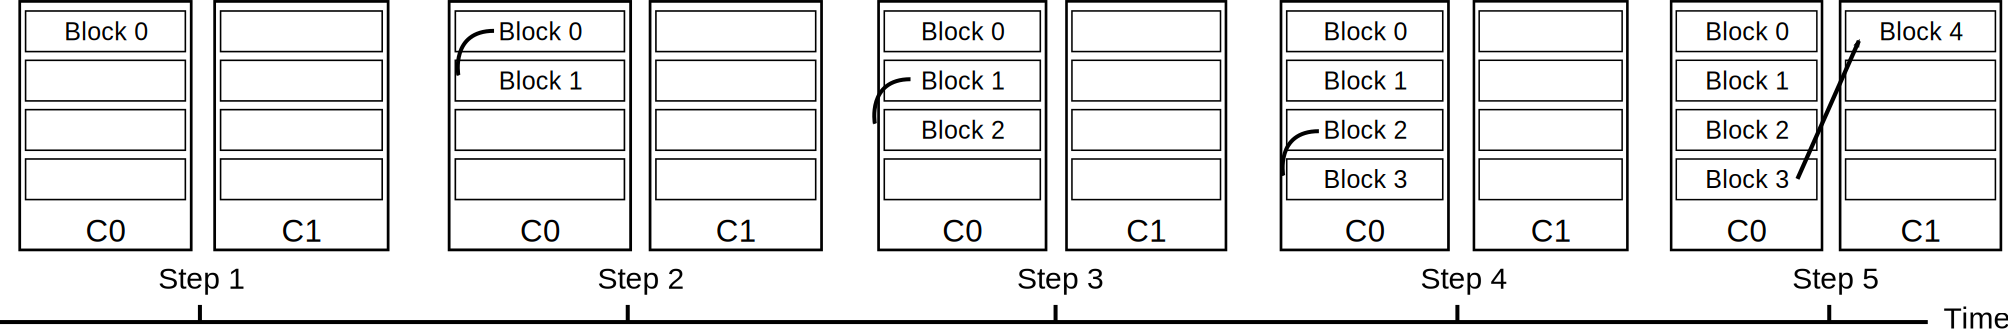
\includegraphics[width=1\textwidth]{chapter3/graphics/normfetch.pdf}
    \caption{Example of the current fetching model on a 2 core composition. Each core has 4 segments, the arrows represent the block generating the predictions. This figure shows the first 5 steps of a new core composition fetching blocks.}
    \label{fig:old_fetch}
\vspace{1em}
\end{figure}
